\section{Kreuz-Prädiktion innere Dynamiken}
\label{sec:exp_inner_prediction}
Bei Messungen der elektrischen Erregung des Herzens können nach aktuellen Stand meistens nur die Erregungen auf der Herzoberfläche gemessen werden. Die Ausbreitungen im Inneren des räumlich ausgedehnten Herzens bleiben somit verborgen. Zudem ist anzunehmen, dass die Gesamtdynamik nicht nur durch die Oberfläche, sondern auch durch die Erregung im Inneren bestimmt und charakterisiert wird. Somit wird die Frage aufgeworfen, ob die innere Erregung des Herzens nur durch die Kenntnis der Oberflächendynamik vorhergesagt werden kann. In diesem Abschnitt soll versucht werden, diese Fragestellung erneut mit den \textsc{ESN}s und den klassischen Methoden zu untersuchen. Dabei wird diese Frage statt an einem dreidimensionalen Systems an den zuvor bereits benutzten zweidimensionalen Modellen untersucht.\\

\begin{figure}[h]
	\centering
	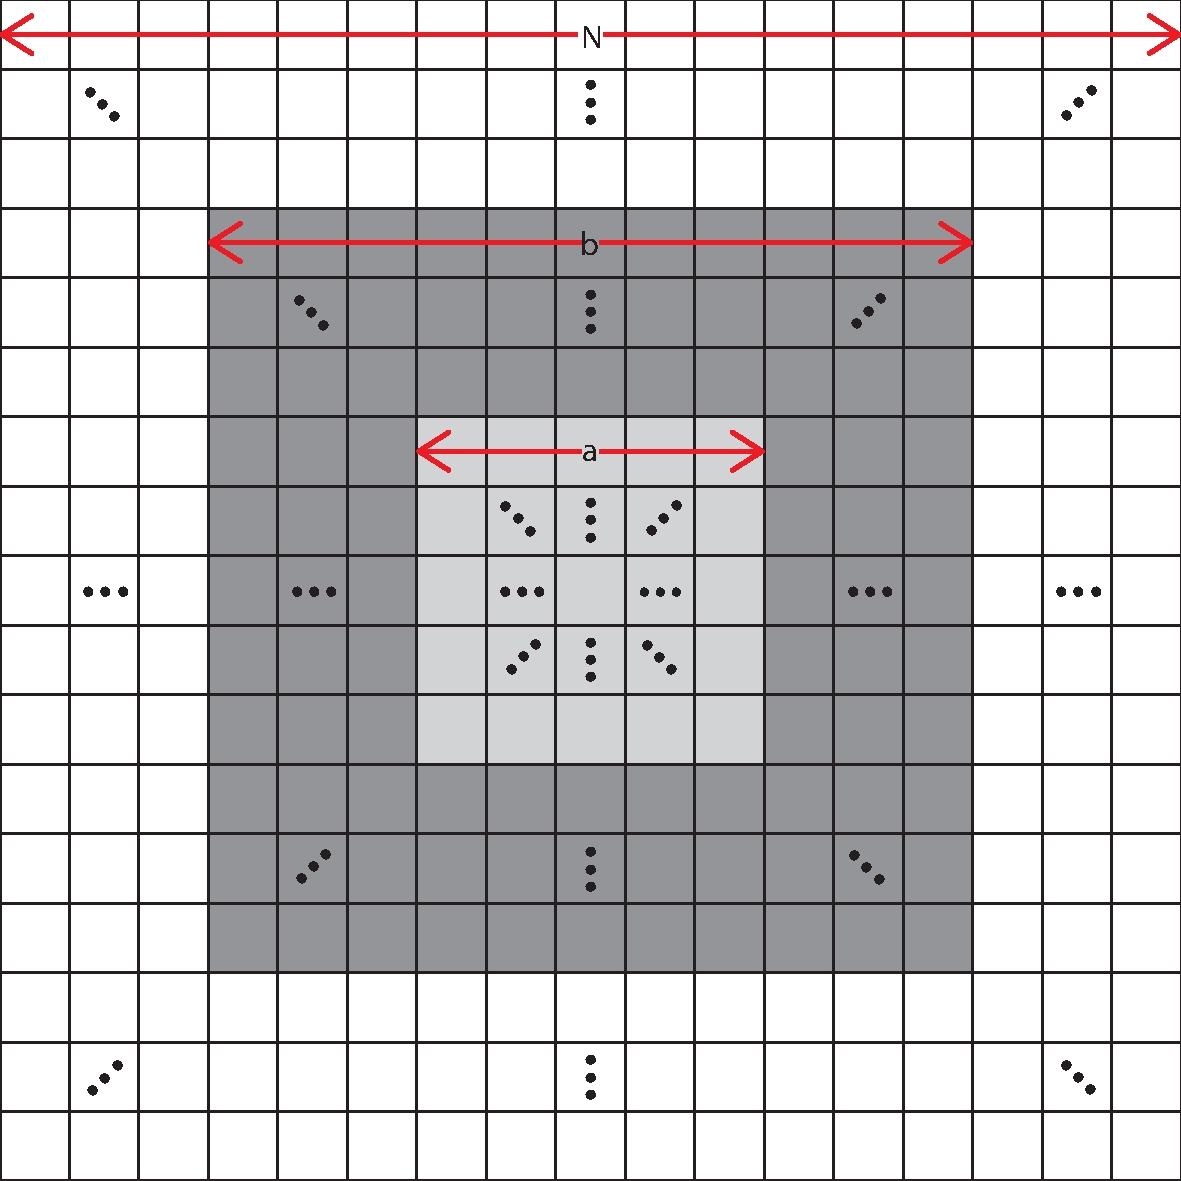
\includegraphics[width=.4\linewidth]{figures/illustrations/inner_prediction.pdf}
	\caption{Darstellung des Aufbaus. Das gesamte $N \times N$ große Feld der Spannungsvariable ist in weiß, wohingegen der vorherzusagende Bereich der Größe $a \times a$ in hellgrau dargestellt ist. Drumherum liegt der dunkelgraue Rahmen der Größe $b \times b$ dessen Pixel für die Vorhersage des Inneren genutzt werden.}
	\label{fig:exp_inner_prediction}
\end{figure}

Hierbei wird nur das Feld der Spannungsvariable betrachtet. In diesem $N \times N$ Einheiten großem Feld wird ein Quadrat mit der Seitenlänge $a$ ausgewählt, für dessen Pixel die Spannungsvariable bestimmt werden soll. Dazu wird um das innere Quadrat ein Rahmen der Breite $b$ gewählt und die Spannungsvariable der beinhalteten Pixel als Quelle genutzt. Eine graphische Illustration dieses Aufbaus ist in Abbildung \ref{fig:exp_inner_prediction} dargestellt. Somit wird die Spannung im Inneren für $a^2$ Punkte durch die Kenntnis der $(a+2b)^2-a^2$ umgebenden Pixel bestimmt.\\

Dieses Szenario ist für die in Tabelle \ref{tab:exp_inner_cross_pred_parameter} angegebenen Parameterkombinationen durchgeführt worden.

\begin{table}[h]
	\centering
	\begin{tabular}{c|c|c|c|c|c|c|c|c|c|c|c|c|c|c|c|c|c|c|c|c|c|}
		$a$ & \multicolumn{3}{c|}{4} & \multicolumn{3}{c|}{8} & \multicolumn{3}{c|}{16} & \multicolumn{3}{c|}{32} & \multicolumn{3}{c|}{64} & \multicolumn{3}{c|}{128*} & \multicolumn{2}{c|}{146*} & 148* \\
		\hline
		$b$ & 1 & 2 & 3 & 1 & 2 & 3 & 1 & 2 & 3 & 1 & 2 & 3 & 1 & 2 & 3 & 1 & 2 & 3 & 2 & 1 & 1 \\
	\end{tabular} 
	\caption{Verwendete Parameter $a$ und $b$ für die Abmessungen des inneren und äußeren Quadrates. Die markierten Werte sind nur für die \textsc{ESN}s untersucht worden.}
	\label{tab:exp_inner_cross_pred_parameter}
\end{table} 

\subsection{Nächste Nachbar Vorhersage}
Für die letzte Aufgabe ist erneut zuerst der \textsc{NN}-Ansatz getestet worden. Es ist anzumerken, dass dies nicht alle Parameterkombinationen $a$, $b$ aus Tabelle \ref{tab:exp_inner_cross_pred_parameter} durchgeführt worden ist, da der Rechenaufwand teilweise zu groß geworden ist. Dies liegt daran, dass die Dimension der Eingabevariablen mit
\begin{align*}
(a+2b)^2-a^2 = 4b^2+4ab
\end{align*}
skaliert. Da zudem die Rechenzeit für diesen Ansatz nach \ref{sc:theory_nn} für wachsende Dimensionen sehr stark zunimmt, kann diese Aufgabe für große Abmessungen des vorherzusagendenen Bereiches nicht mehr in einer angebrachten Zeit berechnet werden.
Die optimalen gefundenen Hyperparameter und die damit erreichten Ergebnisse sind in Tabelle \ref{tab:exp_inner_cross_nn_results} aufgelistet.

\begin{table}[h]
	\centering

	\begin{tabular}{|c|c|c|c|c|c|c|c|c|c|c|}
		\multicolumn{1}{c|}{} & \multicolumn{5}{c|}{Barkley}\\ 
		\hline \hline 
		\rule[-1ex]{0pt}{2.5ex} $a$ & 4 & 8 & 16 & 32 & 64\\ 
		\hline 
		\rule[-1ex]{0pt}{2.5ex} $b$ & 1 & 1 & 1  & 1  & 1 \\ 
		\hline 
		\rule[-1ex]{0pt}{2.5ex} $\delta$ & 4 & 4 & 4 & 3 & 3 \\ 
		\hline 
		\rule[-1ex]{0pt}{2.5ex} k & 5 & 5 & 5 & 5 & 5 \\ 
		\hline 
		\rule[-1ex]{0pt}{2.5ex} Laufzeit [s] & $\approx 1$ & 8 & 287 & 1809 & 14754\\ 
		\hline 
		\rule[-1ex]{0pt}{2.5ex} \textbf{MSE} & \textbf{0.00231} & \textbf{0.00891} & \textbf{0.07097} & \textbf{0.18961} & \textbf{0.24599}\\ 
		\hline 
		\rule[-1ex]{0pt}{2.5ex} \textbf{NRMSE} & \textbf{0.0155} & \textbf{0.0596} & \textbf{0.4779} & \textbf{1.3032} & \textbf{1.7009} \\ 
		\hline 
	\end{tabular} 
	
	\vspace{0.75cm}

	\centering

	\begin{tabular}{|c|c|c|c|c|c|c|c|c|c|c|}
		\multicolumn{1}{c|}{} & \multicolumn{5}{c|}{Mitchell-Schaeffer} \\ 
		\hline \hline 
		\rule[-1ex]{0pt}{2.5ex} $a$ & 4 & 8 & 16 & 32 & 64 \\ 
		\hline 
		\rule[-1ex]{0pt}{2.5ex} $b$ & 1 & 1 & 1  & 1  & 1\\ 
		\hline 
		\rule[-1ex]{0pt}{2.5ex} $\delta$ & 3 & 3 & 3 & 4 & 4 \\ 
		\hline 
		\rule[-1ex]{0pt}{2.5ex} k & 5 & 5 & 5 & 5 & 5 \\ 
		\hline 
		\rule[-1ex]{0pt}{2.5ex} Laufzeit [s] & $\approx 1$ & 17 & 194 & 2482 & 20272\\ 
		\hline 
		\rule[-1ex]{0pt}{2.5ex} \textbf{MSE} & \textbf{0.14221} & \textbf{0.02465} & \textbf{0.06460} & \textbf{0.08744} & \textbf{0.09283} \\ 
		\hline 
		\rule[-1ex]{0pt}{2.5ex} \textbf{NRMSE} & \textbf{0.2663} & \textbf{0.4052} & \textbf{0.9779} & \textbf{1.3564} & \textbf{1.4012} \\ 
		\hline 
	\end{tabular} 

	\caption{Gefundene Hyperparameter der nächsten Nachbar Vorhersage für das \textit{Barkley}-Modell (oben) und das \textit{Mitschell-Schaeffer}-Modell (unten) für verschiedene Größen $a$ des vorherzusagenden Bereichs, welche zu den geringsten Fehlern führen.}
\label{tab:exp_inner_cross_nn_results}
\end{table}

Dabei ist zu erkennen, dass die Qualität der Vorhersage mit steigendem $a$ stark abnimmt. So kann für das \textit{Barkley}-Modell nur für $a \in \{4,8\}$ ein NRMSE der deutlich unter $0.50$ erreicht werden. Für größere Bereiche steigt der NRMSE sogar auf $> 1.0$ an, sodass die Vorhersage nicht besser ist als wenn man den Mittelwert als Vorhersage nimmt. Die Vorhersagen des \textit{Mitchell-Schaeffer}-Modells zeigen eine gleichartige Tendenz, doch starten die Fehler hier bereits deutlich stärker. 

\subsection{Radiale Basisfunktionen}
Analog zu den vorherigen Ausführungen sind die radialen Basisfunktionen ebenfalls auf dieses Problem angewendet worden. Dabei ist mit einer analogen Begründung wie bei den nächsten Nachbarn nur der eingeschränkte Wertebereich für $a$ durchlaufen worden. Die dafür gefundenen Hyperparameter und die Fehler können in Tabelle \ref{tab:exp_inner_cross_rbf_results} gefunden werden.
\begin{table}[h]
	\centering

	\begin{tabular}{|c|c|c|c|c|c|c|c|c|c|c|}
		\multicolumn{1}{c|}{} & \multicolumn{5}{c|}{Barkley}\\ 
		\hline \hline 
		\rule[-1ex]{0pt}{2.5ex} $a$ & 4 & 8 & 16 & 32 & 64\\ 
		\hline 
		\rule[-1ex]{0pt}{2.5ex} $b$ & 1 & 1 & 1  & 1  & 1 \\ 
		\hline 
		\rule[-1ex]{0pt}{2.5ex} $\delta$ & 4 & 4 & 4 & 3 & 3 \\ 
		\hline 
		\rule[-1ex]{0pt}{2.5ex} $\sigma_{RBF}$ & 9 & 5 & 9 & 9 & 7\\ 
		\hline 
		\rule[-1ex]{0pt}{2.5ex} Laufzeit [s] & $\approx 2$ & 7 & 41 & 279 & 1845\\ 
		\hline 
		\rule[-1ex]{0pt}{2.5ex} \textbf{MSE} & \textbf{0.00051} & \textbf{0.00450} & \textbf{0.04009} & \textbf{0.08783} & \textbf{0.13615}\\ 
		\hline 
		\rule[-1ex]{0pt}{2.5ex} \textbf{NRMSE} & \textbf{0.0586} & \textbf{0.1735} & \textbf{0.5196} & \textbf{0.7769} & \textbf{0.9703} \\ 
		\hline 
	\end{tabular} 
	
	\vspace{0.75cm}

	\centering

	\begin{tabular}{|c|c|c|c|c|c|c|c|c|c|c|}
		\multicolumn{1}{c|}{} & \multicolumn{5}{c|}{Mitchell-Schaeffer} \\ 
		\hline \hline 
		\rule[-1ex]{0pt}{2.5ex} $a$ & 4 & 8 & 16 & 32 & 64 \\ 
		\hline 
		\rule[-1ex]{0pt}{2.5ex} $b$ & 1 & 1 & 1  & 1  & 1\\ 
		\hline 
		\rule[-1ex]{0pt}{2.5ex} $\delta$ & 3 & 3 & 3 & 4 & 4 \\ 
		\hline 
		\rule[-1ex]{0pt}{2.5ex} $\sigma_{RBF}$ & 9 & 9 & 9 & 5 & 7 \\ 
		\hline 
		\rule[-1ex]{0pt}{2.5ex} Laufzeit [s] & $\approx 1$ & 7 & 43 & 237 & 1756\\
		\hline 
		\rule[-1ex]{0pt}{2.5ex} \textbf{MSE} & \textbf{0.00064} & \textbf{0.00497} & \textbf{0.02220} & \textbf{0.04745} & \textbf{0.05588} \\ 
		\hline 
		\rule[-1ex]{0pt}{2.5ex} \textbf{NRMSE} & \textbf{0.1094} & \textbf{0.2857} & \textbf{0.5797} & \textbf{0.8580} & \textbf{0.9184} \\ 
		\hline 
	\end{tabular} 

	\caption{Gefundene Hyperparameter der radialen Basisfunktionen für das \textit{Barkley}-Modell (oben) und das \textit{Mitchell-Schaeffer}-Modell (unten) für verschiedene Größen $a$ des vorherzusagenden Bereichs, welche zu den geringsten Fehlern führen.}
\label{tab:exp_inner_cross_rbf_results}
\end{table}

Es ist anzumerken, dass der NRMSE für beide Modelle und alle betrachteten Größen $a$ kleiner als $1.0$ bleibt. Nichtsdestotrotz steigt er ebenfalls mit wachsendem $a$ an, wie schon bei den nächsten Nachbarn. Für die größten beiden $a$-Werte ist in beiden Modellen der Fehler allerdings schon so groß, dass die Vorhersage kaum nützliche Informationen liefert.

\subsection{Echo State Network}
Im Gegensatz zu den anderen beiden Methoden wächst die benötigte Rechenzeit bei der Verwendung der \textsc{ESN}s nicht so schnell an, sodass hiermit auch deutlich größere innere Felder betrachtet werden können. Zur Optimierung des Ansatzes ist erneut das in Abschnitt \ref{sec:exp_general_esn} beschriebene Verfahren durchgeführt worden. Es ist allerdings so modifiziert worden, dass bei der groben Hyperparameterbestimmung des \textsc{ESN} nicht vier statt einem Punkt des inneren Quadrates betrachtet worden sind. Zudem ergibt sich bei dieser Aufgabe ein weiteres Problem, welches eine Modifikation erfordert. In den vorherigen Aufgaben ist die Dimension des Eingangssignals in das \textsc{ESN} $N_u < 50$ gewesen. Nun wächst die Dimension des Eingangssignals allerdings sehr stark mit $N_u = 4b(b+a)$ an. Dies würde bei der Konstruktion der Eingangsmatrix $\mathbf{W_{in}}$ nach Abschnitt \ref{sec:esn_structure} dazu führen, dass die inneren Einheiten des Reservoirs zu viele Eingangssignale erhalten und somit unter Umständen schnell eine Sättigung des $tanh(\cdot)$ in der zeitlichen Entwicklungsgleichung \ref{eq:esn_stateeq} ergibt. Um dies zu lösen ist ein neuer Hyperparameter $FANCY NAME$ eingeführt worden, der die Anzahl von Eingangssignalen pro innerer Einheit beschränkt. Somit wird die Matrix $\mathbf{W_{in}}$ dünn besetzt.\\
Bei der Untersuchung ist ersichtlich geworden, dass der untersuchte Bereich der Regularisierung $\lambda \in [\num{5e-2},\num{5e-6}]$ zu gering ist, da der optimale Wert stets am linken Rand des Intervalls gefunden worden ist. Deswegen ist noch einmal eine Suche auf dem größeren Parameterbereich $\lambda \in [\num{5e-4},\num{5e+4}]$ durchgeführt worden.

\begin{table}[h]
	\centering

	\begin{tabular}{|c|c|c|c|c|c|c|c|}
		\multicolumn{1}{c|}{} & \multicolumn{7}{c|}{Barkley}\\ 
		\hline \hline 
		\rule[-1ex]{0pt}{2.5ex} $a$ & 4 & 8 & 16 & 32 & 64 & 128 & 148\\ 
		\hline 
		\rule[-1ex]{0pt}{2.5ex} $b$ & 1 & 1 & 1 & 1 & 1 & 1 & 1 \\ 
		\hline 
		\rule[-1ex]{0pt}{3.5ex} $N$ & 400 & 400 & 50 & 200 & 400 & 200 & 50\\ 
		\hline 
		\rule[-1ex]{0pt}{3.5ex} $\rho(|\mathbf{W}|)$ & 0.8 & 0.5 & 0.5 & 1.5 & 1.5 & 3.0 & 0.8\\ 
		\hline 
		\rule[-1ex]{0pt}{3.5ex} $\alpha$ & 0.70 & 0.50 & 0.20 & 0.05 & 0.05 & 0.20 & 0.05 \\ 
		\hline 
		\rule[-1ex]{0pt}{3.5ex} $\epsilon$ & 0.2 & 0.2 & 0.1 & 0.2 & 0.2 & 0.2 & 0.1 \\ 
		\hline 
		\rule[-1ex]{0pt}{3.5ex} $\nu_{max}$ & $\num{1e-5}$ & $\num{1e-5}$ & $\num{1e-5}$ & $\num{1e-4}$ & $\num{1e-5}$ & $\num{1e-5}$ &  $\num{1e-5}$\\ 
		\hline 
		\rule[-1ex]{0pt}{3.5ex} $\lambda$ & $\num{5e-4}$ & $\num{5e-1}$ & $\num{5e-1}$ & $\num{5e+3}$ & $\num{5e+4}$ & $\num{5e+3}$ & $\num{5e-6}$\\ 		
		\hline 
		\rule[-1ex]{0pt}{2.5ex} Laufzeit [s] & 5 & 15 & 20 & 131 & 1206 & 3318 & 3010\\
		\hline 
		\rule[-1ex]{0pt}{2.5ex} \textbf{MSE} & \textbf{0.00048} & \textbf{0.00200} & \textbf{0.03460} & \textbf{0.08561} & \textbf{0.15392} & \textbf{0.17220} & \textbf{0.18431}\\ 
		\hline 
		\rule[-1ex]{0pt}{2.5ex} \textbf{NRMSE} & \textbf{0.0179} & \textbf{0.1156} & \textbf{0.4827} & \textbf{0.7671} & \textbf{0.9472} & \textbf{1.0250} & \textbf{1.1153} \\ 
		\hline 
	\end{tabular} 
	
	\vspace{0.75cm}

	\centering

	\begin{tabular}{|c|c|c|c|c|c|c|c|}
		\multicolumn{1}{c|}{} & \multicolumn{7}{c|}{Mitchell-Schaeffer}\\ 
		\hline \hline 
		\rule[-1ex]{0pt}{2.5ex} $a$ & 4 & 8 & 16 & 32 & 64 & 128 & 148\\ 
		\hline 
		\rule[-1ex]{0pt}{2.5ex} $b$ & 1 & 1 & 1 & 1 & 1 & 1 & 1 \\ 
		\hline 
		\rule[-1ex]{0pt}{3.5ex} $N$ & 400 & 50 & 200 & 50 & 400 & 200 & 200\\ 
		\hline 
		\rule[-1ex]{0pt}{3.5ex} $\rho(|\mathbf{W}|)$ & 1.5 & 3.0 & 3.0 & 0.8 & 3.0 & 3.0 & 3.0\\ 
		\hline 
		\rule[-1ex]{0pt}{3.5ex} $\alpha$ & 0.95 & 0.50 & 0.05 & 0.95 & 0.20 & 0.05 & 0.05 \\ 
		\hline 
		\rule[-1ex]{0pt}{3.5ex} $\epsilon$ & 0.1 & 0.1 & 0.2 & 0.1 & 0.1 & 0.1 & 0.2 \\ 
		\hline 
		\rule[-1ex]{0pt}{3.5ex} $\nu_{max}$ & $\num{1e-4}$ & $\num{1e-5}$ & $\num{1e-5}$ & $\num{1e-5}$ & $\num{1e-4}$ & $\num{1e-5}$ &  $\num{1e-5}$\\ 
		\hline 
		\rule[-1ex]{0pt}{3.5ex} $\lambda$ & $\num{5e-0}$ & $\num{5e-2}$ & $\num{5e-1}$ & $\num{5e+3}$ & $\num{5e+3}$ & $\num{5e+4}$ & $\num{5e+4}$\\ 		
		\hline 
		\rule[-1ex]{0pt}{2.5ex} Laufzeit [s] & 5 & 15 & 20 & 131 & 1206 & 3318 & 3010\\
		\hline 
		\rule[-1ex]{0pt}{2.5ex} \textbf{MSE} & \textbf{0.00025} & \textbf{0.00220} & \textbf{0.01889} & \textbf{0.04240} & \textbf{0.05389} & \textbf{0.06596} & \textbf{0.06488}\\ 
		\hline 
		\rule[-1ex]{0pt}{2.5ex} \textbf{NRMSE} & \textbf{0.0687} & \textbf{0.1902} & \textbf{0.5343} & \textbf{0.8110} & \textbf{0.9019} & \textbf{0.9981} & \textbf{0.9844} \\ 
		\hline 
	\end{tabular} 

	\caption{Gefundene Hyperparameter der \textsc{ESN}s für das \textit{Barkley}-Modell (oben) und das \textit{Mitchell-Schaeffer}-Modell (unten) für verschiedene Größen $a$ des vorherzusagenden Bereichs, welche zu den geringsten Fehlern führen.}
\label{tab:exp_inner_cross_esn_results}
\end{table}

Es ist anzunehmen, dass für die Vorhersage eines Punktes der weit von den bekannten Randwerten entfernt liegt, nicht nur durch sein vorheriger Wert und die aktuellen Randwerte benötigt werden. Vielmehr werden die vergangenen Randwerte einen starken Einfluss nehmen. Dies kann an einem Beispiel schnell deutlich gemacht werden: Würde beispielsweise eine ebene Welle durch das Feld propagieren, so können weit entfernte Punkte erst deutlich nachdem die Welle durch die Ränder hindurch gelaufen ist, hiervon beeinflusst werden. Somit benötigt das System eine ausgeprägte Gedächtnisleistung. Bei den \textsc{ESN}s skaliert nach \ref{sc:esn} die Gedächtnisleistung mit der Größe $N$ des Netzwerkes. Es wäre also anzunehmen, dass möglichst große Reservoirs eine optimale Leistung erzielen können. Dies kann experimentell nicht bestätigt werden. So erzielen zwar teilweise die größtmöglichen Reservoirs ($N=400$) die besten Ergebnisse, doch tritt gibt es auch Werte für $a$ bei denen kleinere Reservoirs ($N=50$) besser arbeiten.\\

Hier kann erneut der Trend beobachtet werden, dass der Fehler mit steigendem $a$ ebenso zunimmt. Für das \textit{Mitchell-Schaffer}-Modell sind alle NRMSE-Werte kleiner als $1.0$. Dies ist beim \textit{Barkley-Modell} nicht mehr der Fall für die beiden größten Werte von $a$. 

\subsection{Vergleich}
Für einen Vergleich der drei Methoden bietet es sich an die Ergebnisse für die größten Wert für $a$ durchzuführen, der mit allen drei Ansätzen betrachtet worden ist. Dies entspricht dem Wert $a=64$. Eine Übersicht der verschiedenen Ergebnisse ist in Tabelle \ref{tab:exp_inner_cross_comparison_results} zu finden.

\begin{table}[h]
	\centering
	\captionsetup{width=0.9\linewidth}
	\begin{tabular}{|c|c|c|c|c|c|c|c|}
		\multicolumn{1}{c|}{} & \multicolumn{3}{c|}{Barkley} & \multicolumn{3}{c|}{Mitchell-Schaeffer}		\\
		\cline{2-7}
		\multicolumn{1}{c|}{} & NN & RBF & ESN & NN & RBF & ESN \\
		
		\hline
		\hline
		
		Laufzeit [s] 	& 20272 	& 1756		& \textbf{1089}		& 14754		&  	1845	& \textbf{1206} \\
		\hline
		MSE 			& 0.09284	& 0.05588	& 	\textbf{0.05389} 		& 0.24599	& 0.13615 	& \textbf{0.12975}	 \\
		\hline
		NRMSE 			& 1.1837	& 0.9184	& \textbf{0.9019} 			& 1.3042	& 0.9703 	& \textbf{0.9472} \\
		\hline 
	\end{tabular} 
	\caption{Vergleich der benötigten Laufzeit und der erreichten Fehlers der drei Ansätze für das \textit{Mitchell-Schaeffer}- und das \textit{Barkley}-Modell, welche zu den geringsten Fehlern führen, für $a=64$.}
	\label{tab:exp_inner_cross_comparison_results}
\end{table}

Es zeigt sich erneut, dass die Vorhersagen der klassischen Methoden einen höheren Fehler haben. Während der \textsc{NN}-Ansatz bei beiden Modellen schlechtere Ergebnisse als die Vorhersage mittels des Mittelwertes liefert, sind die radialen Basisfunktionen und die \textsc{ESN}s leicht besser als diese. Dabei erreichen die \textsc{ESN}s und radialen Basisfunktionen in etwa die gleiche Genauigkeit. Diese reicht allerdings auch nicht aus, um dies Methoden tatsächlich sinnvoll verwenden zu können. 

Des Weiteren wächst der Fehlers mit steigender Größe des vorherzusagenden Bereiches auch bei allen drei Ansätze an. Es ist somit zu vermuten, dass dies nicht nur eine reine Beschränkung der einzelnen Methoden ist, sondern dass es womöglich eine Eigenschaft der betrachteten Modelle ist. 
\improvement{Add comparison images}

\begin{figure}[h]
	\centering
	\begin{subfigure}{.5\textwidth}
		\centering
		\includegraphics[height=2.5in]{figures/results/inner_cross_prediction/barkley_u_inner_original.pdf}
		\setcapmargin[1cm]{0.5cm}
		\caption{Echte Erregung des Modells}
		\label{fig:exp_inner_cross_barkley_result_orig}
	\end{subfigure}%
	\begin{subfigure}{.5\textwidth}
		\centering
		\includegraphics[height=2.5in]{figures/results/inner_cross_prediction/barkley_u_inner_nn.pdf}
		\setcapmargin[1cm]{0.5cm}
  		\caption{Vorhersage des \textsc{NN}-Ansatzes}
  		\label{fig:exp_inner_cross_barkley_result_nn_pred}
	\end{subfigure}
	\begin{subfigure}{.5\textwidth}
		\centering
		\includegraphics[height=2.5in]{figures/results/inner_cross_prediction/barkley_u_inner_rbf.pdf}
		\setcapmargin[1cm]{0.5cm}
  		\caption{Vorhersage des \textsc{RBF}-Ansatzes}
  		\label{fig:exp_inner_cross_barkley_result_rbf_pred}
	\end{subfigure}%
	\begin{subfigure}{.5\textwidth}
		\centering
		\includegraphics[height=2.5in]{figures/results/inner_cross_prediction/barkley_u_inner_esn.pdf}
		\setcapmargin[1cm]{0.5cm}
  		\caption{Vorhersage des \textsc{ESN}}
  		\label{fig:exp_inner_cross_barkley_result_esn_pred}
	\end{subfigure}
	\caption{Graphische Darstellung der $u$-Variable des \textit{Barkley}-Modells für den $1000$. Zeitschritt des Testdatensatzes. Oben links ist das tatsächliche Feld des Modells zu sehen. Danach folgenden im Uhrzeigersinn die Vorhersagen des \textsc{NN}-Ansatzes, des \textsc{RBF}-Ansatzes und des \textsc{ESN}.}
	\label{fig:exp_inner_cross_barkley_result}
\end{figure} 

In Abbildung \ref{fig:exp_inner_cross_barkley_result} werden exemplarisch die aus den drei Ansätzen resultierenden Felder der Spannungsvariable $u(t)$ des \textit{Barkley}-Modells zusammen mit dem originalen Feld dargestellt. Hierbei fällt auf, dass sowohl die Vorhersage der \textbf{RBF} als auch die des \textit{ESN} stark verschwommen sind und kaum Details zeigen. Im Gegensatz dazu gibt der \textit{NN}-Ansatz eine sehr scharfe Vorhersage. Dies ist dahingehend interessant, als das zum einen jeder Bildpunkt einzeln vorhersagt wird, und zum anderen immer die nächsten fünf Nachbarn genutzt werden. Daraus können zwei Konsequenzen folgen. Erstens spricht die hohe Auflösung dafür, dass die Vorhersage beinahe perfekt ein Bereich aus den Trainingsdaten ist. Da die Vorhersage aber (zumindest in diesem Moment) nicht gut mit dem Original übereinstimmt bedeutet dies, dass die Verzögerungskoordinaten, die genutzt worden sind, den Bereich nicht eindeutig beschreiben. Zweitens kann daraus auch gefolgert werden, dass für diese Aufgabe die Länge der Trainingsdaten zu gering gewählt worden ist. 
